\documentclass[12pt, a4paper]{report}
\usepackage{svg}
\usepackage{wrapfig}
\makeatletter
 \newcommand\wrapfill{\par
   \ifx\parshape\WF@fudgeparshape
   \nobreak
   \vskip-\baselineskip
   \vskip\c@WF@wrappedlines\baselineskip
   \allowbreak
   \WFclear
   \fi
 }
\usepackage[font=footnotesize]{caption}
\usepackage[margin=.5in]{geometry}
\usepackage{hyperref}
\usepackage{forest}
\usepackage{lipsum}
\usepackage{color}
\usepackage{listings}
\usepackage{listings-rust}
\usepackage{xcolor}
\usepackage{graphicx}
\graphicspath{ {./pictures/} }
\definecolor{codegreen}{rgb}{0,0.6,0}
\definecolor{codegray}{rgb}{0.5,0.5,0.5}
\definecolor{codepurple}{rgb}{0.58,0,0.82}
\definecolor{backcolour}{rgb}{1,1,1}

\lstdefinestyle{mystyle}{
    backgroundcolor=\color{backcolour},   
    commentstyle=\color{codegreen},
    keywordstyle=\color{magenta},
    numberstyle=\tiny\color{codegray},
    stringstyle=\color{codepurple},
    basicstyle=\ttfamily\footnotesize,
    breakatwhitespace=false,         
    breaklines=true,                 
    captionpos=b,                    
    keepspaces=true,                 
    numbers=left,                    
    numbersep=5pt,                  
    showspaces=false,                
    showstringspaces=false,
    showtabs=false,                  
    tabsize=2
}

\lstset{style=mystyle}

\setlength{\intextsep}{0mm}
\svgpath{{svg/}}
\svgsetup{inkscapelatex=false}

\begin{document}
\title{NEA Documentation}
\author{Hugh O'Donnell}
\date{November 2022}
\maketitle
\tableofcontents
\chapter{Analysis}
\section{My Project}
Othello is an abstract strategy game played on an 8 by 8 board.
I will implement a digital version of Othello with a graphical user interface and a computer player.
The end user will be Eugene O'Donnell.
\section{Othello}
\subsection{Rules}
\wrapfill
	
\begin{wrapfigure}{r}{0pt}
	\centering
	\includesvg[width=.28\textwidth]{initial_othello}
	\caption{An Othello board's starting position. By convention, the black piece closest to each player is on that player's left,
	although this is inconsequential due to symmetry.}
	\label{fig:init}
\end{wrapfigure}

Othello is an abstract strategy game. Two players, black and white, play against each other on an 8 by 8 board placing one disc on each turn.
Players alternate turns with black moving first. If a player has no legal moves and it is their turn, it is the other player's turn again.
If both players have no legal moves, the game ends, and the winner, if they exist, is the player with the most discs of their colour on the board.
If the winner does not exist, i.e., when there are the same number of black discs and white discs on the board, the game ends in a draw.


When a player makes a move, they place a disc on the board with their colour facing upwards.
If there is a continuous line of discs of the opposing colour between the disc just placed and another disc of the player’s colour, those discs of the opposing colour are captured (flipped), and thus changed to the colour of the player who made the move.
If, and only if, a move causes discs to be flipped, that move is legal.
The official rules are here: \url{https://www.worldothello.org/about/about-othello/othello-rules/official-rules/english}.
\wrapfill

\begin{wrapfigure}[9]{l}{0pt}
	\centering
		\includesvg[width=.28\textwidth]{move_example}
		\caption{The position in~\ref{fig:init} if black plays E6}
\end{wrapfigure}

\subsection{Computer Othello}

Almost all algorithms for estimating a good move for an abstract strategy game such as Othello involve an inexhaustive search of the game tree.
The game tree consists of nodes which represent different Othello positions, and edges from parent nodes to child nodes
represent the fact that the position which the child node represents can be reached in exactly one move from the position
represented by the parent node.
An evaluation function, i.e., a function of a position which evaluates how advantageous that position is to a particular player,
is common to many, but not all, game-playing algorithms. 

\subsubsection{Minimax}

Minimax is a brute force algorithm for searching the game tree, parameterized by an evaluation function, \(f\) and a search depth, \(n\).
All of the possible positions after \(n\) moves will be evaluated with \(f\).
The move which \em guarantees \em the most advantageous position (the one with the greatest evaluation) is chosen.
Minimax at depth \(n\) has time complexity \(\mathcal{O}(b^n)\) and space complexity \(\mathcal{O}(bn)\), where \(b\) is the branching factor,
i.e., the average number of legal moves in an Othello position, which for Othello is about 10. Many of the other
algorithms for finding a good move are similar to minimax.
I will use minimax with a variation of alpha-beta pruning in order
to find the best move given some particular Othello position.
Alpha-beta pruning is purely an optimization of minimax; it does not change the result.
As minimax is better at greater depths, the depth
can serve as a difficulty which the end user can adjust.
\wrapfill

\begin{figure}[h]
	\centering
	\begin{forest}
		[\includesvg{initial_othello}
			[\includesvg{m3}]
			[\includesvg{move_example} [\includesvg{m4}], [\includesvg{m5}]]
		]
	\end{forest}
	\caption{A small subgraph of Othello's game tree. The size of the whole tree is estimated at \(10^{54}\) nodes.}
\end{figure}


\subsubsection{Evalutaion Functions}

The evaluation function is crucial to the strength of the computer player; it is far more important than the search function.
There are several ways to evaluate an othello position. I will discuss two below.

\paragraph{Disc-Square Tables:}

A disc-square table assigns some value to each square on an Othello board, with squares with higher values being better squares
to have a piece on. The value of a position can be calculated by subtracting the sum of
the squares which white occupies from the sum of those which black occupies. The table can be changed between stages of the game
because the most important squares to occupy change over the course of the game.

\paragraph{Mobility-Based Evaluation:}

This evaluation function gives preference to positions with more available moves and fewer frontier discs, i.e., discs adjacent to
empty squares. In Othello, there is no stalemate; if a player has no legal moves, they forfeit their turn, which is unfavourable
and something which this evaluation function optimizes for. Mobility-based evaluation is generally better than disc-square tables because
the mobility of a player's position changes less from turn to turn than the score from a disc-square table, as rows of discs can be
flipped which drastically changes the disc-square table evaluation.
\\ \\
I will use a combination of both methods.
I will value occupance of the corners, everything else will be mobility-based evaluation.
It is impossible to flip a disc at one of the corners so this method does not succumb the aforementioned shortcoming of a disc-square table. 


\section{End User and Requirements}
The end user is Eugene O'Donnell, my father.
He wants a digital implementation of Othello because it is easier to play against a computer than to find a human to play against and carry the board and pieces around.
From conversations with him about the project, I have compiled the following list of requirements:
\begin{enumerate}
\item A digital Othello board on which the user can click on a square to place a disc there.
\item Show the number of discs each player has next to the board.
\item A computer player with an adjustable difficulty, which is strong enough to beat the supervisor without taking more than five seconds for any single move.
\item An option to change the colours used to draw the board and discs with colour pickers.
\item An option to choose between playing as black or white.
\item All of a player's legal moves should be shown on the board.
\end{enumerate}

\section{Proposed Solutions}
Here are my evaluations and decisions over how I will solve the objectives.
\subsection{Programming Language}
I know Python and C++ well enough for this project.
I am also considering using Rust, although my knowledge of it is limited, because it is memory safe and about as fast as C++.
I know I will have to use multi-threading in some capacity in order to have the GUI (Graphical User Interface) respond while the minimax is running.
I want the minimax to run as fast as possible in order to search as far ahead as possible within a reasonable amount of time.
\subsubsection{Advantages and Disadvantages}
\begin{tabular}{| p{0.3\textwidth} | p{0.3\textwidth} | p{0.3\textwidth} |}
	\hline
	 	Python                  & C++                      & Rust                      \\ \hline
	 	\begin{enumerate}
		 	\item[+] Memory safe (garbage collected).
		 	\item[+] I have experience.
		 	\item[+] Interpreted, so more portable than Rust or Python.
		 	\item[-] Interpreted, so executes relatively slowly.
	 	\end{enumerate}
	 	& \begin{enumerate}
		 	\item[+] Fast.
		 	\item[+] I have experience.
		 	\item[+] Statically typed.
		 	\item[-] Code must be compiled each time, which can take a long time.
		 	\item[-] Not memory safe, so bugs are more easily created.
	 	\end{enumerate}
	 	& \begin{enumerate}
	 		\item[+] Memory safe (borrow checker), in fact data races are impossible.
	 		\item[+] Fast.
	 		\item[+] Statically typed.
	 		\item[-] Code must be compiled each time, and the compilation is slower than in C++.
	 		\item[-] I don't have much experience.
	 		\item[-] There are fewer libraries available than in Python or C++
	 	\end{enumerate}
	\\ \hline
\end{tabular}
\\ \\
I have decided to go with Rust, because I want to learn it and the impossibility of data races eliminates a whole class of bugs which could be introduced in the implementation of multithreading.

\subsection{Graphical User Interface Library}
I decided to use FLTK because there are not too many GUI libraries for Rust, and this one seemed to be well documented and well used, as it was originally a C++ library.
I do not know that much about all the other GUI libraries because I have not tried many of them, but FLTK works well enough for me so I will use it.

\section{Objectives}
Here are my objectives, based on the end user's requirements:
\begin{enumerate}
	\item Upon launching the program, a graphical user interface should be shown to the user.
	\item When playing Othello, a disc should be placed on the board when a square is clicked if and only if it is the human player's turn, and the move which they are making is legal.
	\item The difficulty of the computer player must be selectable through the graphical user interface.
	\item The colour of the human must be selectable through the graphical user interface.
	\item The user must be able to choose the colour of the discs and squares on the board with a colour picker.
	\item The computer player must make moves good enough to beat the end user, taking no longer than five seconds to make one move.
	\item The graphical user interface should display the number of discs belonging to each player on the board.
	\item When the game is over, the graphical user interface should show whether the game was won or drawn, and if the game was won, which player won.
	\item The graphical user interface must remain responsive while the computer player is computing a move.
\end{enumerate}

\chapter{Documented Design}
I will explain the data structures I used first, then the algorithms. This is because an understanding of the data structures used is needed to understand some of the algorithms.

\section{Software Architecture}
There are two main responsibilities of my software; I need to implement a digital representation of an Othello board with a strong computer player, and I need to implement a GUI which will
allow my client to play against the computer. The digital representation of Othello should know nothing of the GUI, but the code for the GUI will have to know how the board is represented,
how a move is represented etc. in order to draw the board and allow the player to make moves. For this reason, I wrote the digital representation of Othello before writing the GUI.

\section{Data Structures for Othello}
Here I will explain all of the types I defined for the digital representation of Othello, but \emph{not} for the GUI.

\subsection{\texttt{BoardState}}
A variable of type \texttt{BoardState} is either \texttt{BoardState::Won}, \texttt{BoardState::Drawn}, or \texttt{BoardState::Ongoing}. \texttt{BoardState} is implemented as an \texttt{enum} like so:

\begin{lstlisting}[language=Rust]
#[derive(Clone, PartialEq, Debug, Copy)]
pub enum BoardState {
    Won, // to_move has won, so we don't need a `BoardState::Lost`
    Drawn,
    Ongoing,
}
\end{lstlisting}

the first line tells Rust to automatically implement some useful methods.

\subsection{Bitboards}
The pieces on the board can be thought of as an eight by eight 2D array with each row in the 2D array representing a row of eight squares on the board, with each element of that row representing either an empty square, a black disc, or a white disc.
One could then imagine doing away with the 2D array and instead using a 1D array, with the boundary of each row being managed by the programmer. The square at the \(i^{\textrm{th}}\) column and the \(j^{\textrm{th}}\) row
would be the \((8i + j)^{\textrm{th}}\) (or the \((i + 8j)^{\textrm{th}}\) - this is inconsequential as long as a choice is made and stuck to) element of the 1D array. This is more space efficient than the 2D array because a (64 bit) pointer
to the head of each array must be stored in memory. With the 2D array version there are nine arrays in total, whereas with the 1D case there is only one array. It is also faster to access individual elements in the 1D array because
all of the elements are stored contiguously in memory and accessing an individual element requires only one pointer dereference, instead of the two required in the 2D case (one for the row array, and one to read an element of that row array).
Each element of this array can represent one of three things, as mentioned earlier: an empty square, a black disc, or a white disc. This means that each element must take up at least \(\lceil\log_{2}3\rceil = 2\) bits in memory.
If two 64-bit integers (128 bits in total) are used (it is more helpful to think of them as 64-bit blocks of memory which happen to support bitwise logic operations and shifts), the same information can be encoded if in one of the
integers the location of the black discs is stored, the locations of white discs in the other. This is called a bitboard. This also allows useful information about the board to be computed very quickly with bitwise operations and shifts, 
e.g. the locations of the empty squares can be computed by ANDing the bitwise NOT of the black and white squares.

\subsection{\texttt{Pieces}}
\label{pieces}
The \texttt{Pieces} struct is a wrapper for an unsigned 64-bit integer, on top of which I have implemented the \texttt{Iterator} trait which allows me to iterate over each bit in the integer.

\begin{lstlisting}[language=Rust]
#[derive(Clone, Copy)]
pub struct Pieces {
    pub bits: u64,
}

impl Iterator for Pieces {
    type Item = u64;
    fn next(&mut self) -> Option<Self::Item> {
        if self.bits == 0 {
            None
        } else {
            let bit = self.bits ^ (self.bits & (self.bits - 1));
            self.bits &= self.bits - 1;
            Some(bit)
        }
    }
}
\end{lstlisting}

\texttt{Iterator} is a trait (similar to an interface) defined in Rust's standard library which can be implemented by defining the \texttt{next} method. Implementing \texttt{Iterator} for a type allows 
objects of that type to be used in for loops, and gives the programmer access to many other methods, e.g. \texttt{filter} and \texttt{map}. 
The \texttt{next} method returns the least significant bit and mutates the inner integer. This is all that is required to be able to iterate over each piece in an object which is of type \texttt{Pieces}, 
and all the methods on a type which implements the \texttt{Iterator} trait are available.
When the object has no pieces left, i.e., \texttt{self.bits == 0}, a null value is returned, which is expressed in the return type of the method which is \texttt{Option<Self::Item>} and not just \texttt{Self::Item}.
In \texttt{Self::Item}, \texttt{Self} is a synonym for \texttt{Pieces}, and \texttt{Item} is defined as an unsigned 64-bit integer on the seventh line.

\subsection{\texttt{Board}}
The \texttt{Board} struct combines the \texttt{Pieces} and \texttt{BoardState} types to store the state of an Othello board, using bitboards. There is also a flag, \texttt{black\_moving} which indicates which colour is moving.

\begin{lstlisting}[language=Rust]
#[derive(Clone, Copy)]
pub struct Board {
    pub to_move: Pieces,
    pub waiting: Pieces,
    pub black_moving: bool,
    pub board_state: BoardState,
}
\end{lstlisting}

\section{Algorithms for Othello}
Here I will explain all of the functions I defined when writing the digital representation of Othello.

\subsection{Implementation of \texttt{std::default::Default} for \texttt{Board}}
\texttt{std::default::Default} is a trait in Rust's standard library which requires one method, \texttt{default}, and only exposes one method, \texttt{default}. The \texttt{default} method is a constructor for the type which 
implements it, conventionally returning a "default" object of that type. In my case, I have implemented \texttt{default} to return an Othello board in a game's initial position, like the one shown in \ref{fig:init}.

\begin{lstlisting}[language=Rust]
impl Default for Board {
    fn default() -> Self {
        Board {
            black_moving: true,
            board_state: BoardState::Ongoing,
            waiting: Pieces {
                bits: 0b1000000001000000000000000000000000000,
            },
            to_move: Pieces {
                bits: 0b100000010000000000000000000000000000,
            },
        }
    }
}
\end{lstlisting}

The bits field is filled in for each colour in the starting position of an Othello board, which I worked out using an online bitboard viewer: \url{https://tearth.dev/bitboard-viewer/}.
In Othello black moves first, so the \texttt{black\_moving} field is set to \texttt{true}. Because 

\subsection{Implementation of \texttt{std::fmt::Debug} for \texttt{Board}}

\begin{wrapfigure}{r}{0pt}
	\centering
	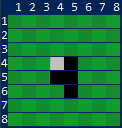
\includegraphics{debug_impl}
	\caption{This is what my implementation of \texttt{Debug} prints when called.}
\end{wrapfigure}

\texttt{std::fmt::Debug} is a trait, which when implemented for a type allows objects of that type to be printed to the terminal for debugging purposes. I could have used the defualt implementation with 
\texttt{\#[derive(Debug)]} above the declaration of \texttt{Board}, but this would print the fields of the board one-by-one, so I would not be able to easily tell the state of my board and see if anything unexpected
was happening before I implemented my GUI. By implementing the \texttt{Debug} trait myself, I can get a graphical visualization of the current state of the board in the terminal by printing coloured block characters.

\subsection{Implementation of \texttt{Board::each\_move}}
\texttt{Board::each\_move} is one of the methods of \texttt{Board}. It takes a read-only reference to the object of type \texttt{Board} which it is called on, and returns a \texttt{Pieces} object representing the locations
of all the legal moves on the current state of the board.

\begin{centering}
\texttt{                          \\
63 62 61 60 59 58 57 56 \\
55 54 53 52 51 50 49 48 \\
47 46 45 44 43 42 41 40 \\
39 38 37 36 35 34 33 32 \\
31 30 29 28 27 26 25 24 \\
23 22 21 20 19 18 17 16 \\
15 14 13 12 11 10 09 08 \\
07 06 05 04 03 02 01 00 \\
}
\end{centering}
These are the indices of each bit in the 64-bit bitboard when arranged into an eight by eight grid, like in Othello. Given the index of some square on the board, it would be useful to be able to find the index of 
the adjacent squares. To move:
\begin{description}
	\item[North] Add eight to the index.
	\item[North-East] Add seven to the index.
	\item[East] Subtract one from the index.
	\item[South-East] Subtract nine from the index.
	\item[South] Subtract eight from the index.
	\item[South-West] Subtract seven from the index.
	\item[West] Add one to the index.
	\item[North-West] Add nine to the index.
\end{description}
The bits of the bitboard can be shifted all at once with a bitshift in any of these directions. If the index is added to then a left shift is used, and if the index is subtracted from then a right shift is used.
This is used to compute the legal moves given some position in \texttt{Board::each\_move} efficiently, as will be explained shortly.

\subsubsection{What constitutes a legal move?}
As mentioned earlier, a move is legal if and only if it flips some of the opponent's discs. Suppose there two players, white and black, with white to move. A black disc will be flipped after white's move
if and only if there is a straight or diagonal path ending where there are no more black discs, with one end at the newly placed white disc, and the other end at a preexisting white disc. In other words, for a move to be legal, 
there must exist a line starting at the newly placed disc, ending at a disc of the same colour, and passing only through discs of the opposition's colour. This implies that the newly placed disc is adjacent to at least one disc 
of the opposing colour. The newly placed disc must also be on an empty square. The empty squares neither of either players' discs on them, so can be computed quickly like so: 
\begin{lstlisting}[language=Rust]
let empty = !(friend | opponent)
\end{lstlisting}
where \texttt{friend} is the bitboard containing the discs of the player to move, and \texttt{opponent} are the discs of the opponent.

\subsubsection{The Code}
\begin{lstlisting}[language=Rust]
impl Board {
    // The second item of each tuple are the squares where you shouldn't shl from for each dir
    pub const DIRECTIONS: [(i8, u64); 8] = [
        (8, 0),
        (9, 0x8080808080808080),
        (1, 0x8080808080808080),
        (-7, 0x8080808080808080),
        (-8, 0),
        (-9, 0x0101010101010101),
        (-1, 0x0101010101010101),
        (7, 0x0101010101010101),
    ];
    pub fn each_move(&self) -> Pieces {
        let (friend, opponent) = (&self.to_move.bits, &self.waiting.bits);
        let safe_shl = |a: u64, b: i8| if b > 0 { a << b } else { a >> (-b) };
        let mut moves: u64 = 0;
        let empty = !(friend | opponent);
        for (dir, guard) in Board::DIRECTIONS {
            let mut candidates = opponent & safe_shl(*friend & !guard, dir);
            while candidates != 0 {
                moves |= empty & safe_shl(candidates & !guard, dir);
                candidates = opponent & safe_shl(candidates & !guard, dir);
            }
        }
        Pieces { bits: moves }
    }
}
\end{lstlisting}

\texttt{DIRECTIONS} is an array of tuples containg a direction and a guard. The direction is the value by which a set of bits should be left shifted to slide north, north-west, west, etc., and the guard is a set of bits which should never be shifted 
in that direction, lest they wrap around. For example, consider a bit on the left edge of the board (not the top left though). If this bit is left shifted by one, It will move one row up and onto the right edge of the board, not to the west.
This is undesirable, so any bits about do be shifted in a given direction should be intersected (bitwise AND) with \texttt{!guard}.

\texttt{safe\_shl} is a closure (similar to a function, very similar to a lambda) allowing me to left shift by a negative number of bits, which the left shift operator does not allow in Rust. If I want to left shift \texttt{a} by \texttt{b} bits, I check if \texttt{b} is negative, and 
if so, I right shift \texttt{a} by \texttt{-b} bits for the desired behaviour.

\texttt{friend} is the bitboard containing the discs of the player about to move, and \texttt{opponent} is the bitboard with their opponent's discs.

\texttt{moves} is an unsigned 64-bit integer which I use to accumulate the legal moves.

For each \texttt{dir} (direction), I generate a set of candidates, which are squares which could be one square from a legal move in the direction currently being considered. If a candidate is one square away from an empty square in the current 
direction, that empty square is legal to move on, so I add it to the moves. I do this until there are no more candidates, and then start on the next direction until all the directions have been considered, at which point I return the moves, wrapped 
in a \texttt{Pieces} object (\texttt{struct Pieces} is explained in \ref{pieces}).
\\

\begin{figure}[h]
	\centering
	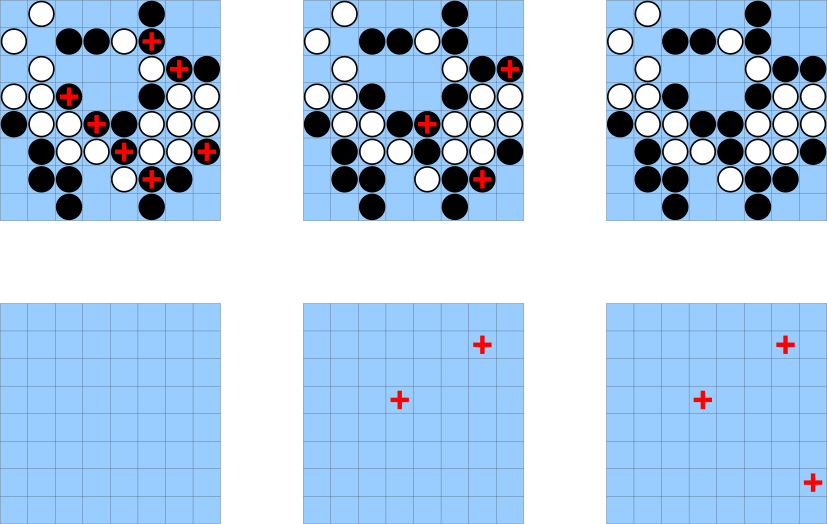
\includegraphics[width=.75\textwidth]{bitmap}
	\caption{Legal moves for white which have been generated by shifting east. The top row shows the discs and the red crosses are the candidates. The bottom row shows the legal moves which have been accumulated .}
\end{figure}

\subsection{Implementation of \texttt{Board::make\_move}}
This method takes a mutable reference to a \texttt{Board} object, and a bit which is passed as an unsigned 64-bit integer (the integer should be of the form \(2^k, 0 <= k <= 63\)), 
which is the move to be made. It is not passed as an index, despite the fact that this would only use one byte instead of eight, because the caller of this method will usually have the move stored as an unsigned 64-bit 
integer and so having to convert the move back to an index at the call site, and back to a 64-bit integer in the function, is avoided.

First, the opponent's discs which will be flipped are computed. This is done by sliding a copy of the bit passed to the function in each direction until it is no longer at one of the opponent's discs, 
and flipping the discs it passes over if the last square it lands on is not one of the opponent's discs and not an empty square. Then comes the slightly cumbersome process of determing who should move next.
As mentioned previously, if a player has no legal moves, it becomes their opponent's turn, and if the opponent also has no legal moves, the game ends in a win for the player with more discs of their colour on the board.
If there are an equal number of discs of each colour on the board, the game ends in a draw. Because the legal moves have to be computed in order to determine who's turn it is after the move, the legal moves are returned 
because they are also often required by the caller, which avoids wasting time computing the legal moves twice.

\subsubsection{The Code}
\begin{lstlisting}[language=Rust]
pub fn make_move(&mut self, bit: u64) -> Pieces {
    // Returning the moves because the caller often needs it anyway
    let safe_shl = |a: u64, b: i8| if b > 0 { a << b } else { a >> (-b) };
    for (dir, guard) in Board::DIRECTIONS {
        let mut line = 0u64;
        let mut moving_bit = safe_shl(bit & !guard, dir);
        while moving_bit & self.waiting.bits != 0 {
            line |= moving_bit;
            moving_bit = safe_shl(moving_bit & !guard, dir);
        }
        if moving_bit & self.to_move.bits != 0 {
            self.to_move.bits |= line;
            self.waiting.bits &= !line;
        }
    }
    self.to_move.bits |= bit;
    std::mem::swap(&mut self.to_move, &mut self.waiting);
    self.black_moving ^= true;
    let mut moves = self.each_move();
    self.board_state = if moves.bits == 0 {
        std::mem::swap(&mut self.to_move, &mut self.waiting);
        self.black_moving ^= true;
        moves = self.each_move();
        if moves.bits == 0 {
            use std::cmp::Ordering;
            // No possible moves for both sides
            match self
                .to_move
                .clone()
                .count()
                .cmp(&self.waiting.clone().count())
            {
                Ordering::Greater => BoardState::Won,
                Ordering::Less => {
                    std::mem::swap(&mut self.to_move, &mut self.waiting);
                    self.black_moving ^= true;
                    BoardState::Won
                }
                Ordering::Equal => BoardState::Drawn,
            }
        } else {
            BoardState::Ongoing
        }
    } else {
        BoardState::Ongoing
    };
    moves
}
\end{lstlisting}

\texttt{safe\_shl} is defined in the same way again to allow left shifting by a negative number of bits. Once the discs have been flipped, it becomes the opponent's turn with \texttt{self.black\_moving \^{}= true;}. 
The \texttt{\^{}} operator means XOR. The legal moves for the opposition are computed with \texttt{let mut moves = self.each\_move();}, and if there are no legal moves for the opposition, it becomes the other player's turn again, 
and if that player has no legal moves either, the game is over and the winner is determined by counting the number of discs each player has.

\subsection{Implementation of \texttt{Board::safe\_make\_move}}
This method is very simple. Its parameters are the same as \texttt{Board::make\_move}, but before making the move, the legality of the move is confirmed. The move is made in the same way as \texttt{Board::make\_move} only if the move 
is legal. If the move is illegal, the move is not made.

\subsubsection{The Code}
\begin{lstlisting}[language=Rust]
pub fn safe_make_move(&mut self, bit: u64) -> Result<Pieces, String> {
    let mut moves = self.each_move();
    match moves.any(|x| x == bit) {
        true => {
            self.make_move(bit);
            Ok(moves)
        }
        false => Err(String::from("Move is not legal")),
    }
}
\end{lstlisting}

The return type \texttt{Result<Pieces, String>} is used because the function can fail, so the caller should be able to tell whether the function failed by checking which variant of the \texttt{Result} enum is returned. 
If the move is illegal, the string "Move is not legal" is returned, wrapped in the \texttt{Err} variant of the \texttt{Result} enum, 
otherwise, the legal moves are returned wrapped in the \texttt{Ok} variant of the \texttt{Result} enum.
\texttt{moves.any{|x| x == bit}} evaluates to a boolean; true if any of the legal moves in the position are equal to the move (\texttt{bit}) passed to the function, and false if not.

\subsection{Implementation of \texttt{Board::children}}
This method takes a bitboard containing all the legal moves in a position, and returns a vector of tuples. The first item of the \(k^\textrm{th}\) tuple is the state of the board after having made the \(k^\textrm{th}\) legal move.
The second item of each tuple is the set of legal moves in the position after having made the move. The set of legal moves for each child is returned because it must be computed anyway and very likely to be needed by the caller,
so it would be a waste not to return it. The legal moves are passed in as an argument, despite being completely dependent on the board (the first argument), because the caller is likely to have computed them beforehand, 
so, again, this in order to avoid doing unnecessary computation.

\subsubsection{The Code}
\begin{lstlisting}[language=Rust]
pub fn children(&self, moves: &Pieces) -> Vec<(Board, Pieces)> {
    // Moves is a parameter as the caller will often already have calculated it
    // Returning both positions and the available moves as the latter
    // must be calculated and I don't want to waste the computation
    moves
        .clone()
        .map(|bit| {
            let mut next_board = self.clone();
            let next_board_moves = next_board.make_move(bit);
            (next_board, next_board_moves)
        })
        .collect()
}
\end{lstlisting}

\texttt{map} is a function in \texttt{Iterator}'s interface. It takes the implicitly passed object which implements \texttt{Iterator} and a closure, and returns a \texttt{Map} object. The fine details of this \texttt{Map} object are 
irrelevant, and at a basic level it is helpful to think of it as being synonymous with a \texttt{Vec}. In each element of the returned \texttt{Map} object is the value returned by the closure applied to the element at that position 
in the vector. \texttt{collect} is another function in \texttt{Iterator}'s interface. In this context, it just converts the \texttt{Map} object into a \texttt{Vec}.

\subsection{Implementation of \texttt{frontier}}
\texttt{frontier} is a function which takes a \texttt{Board} object as its single argument, and returns a tuple containing two \texttt{Pieces} objects.

\end{document}

















